\documentclass[12pt,a4paper]{article}

\usepackage[T1]{fontenc}
\usepackage{lmodern}
\usepackage[utf8]{inputenc}
\usepackage[czech]{babel}
\usepackage[a4paper,margin=2.5cm]{geometry}
\usepackage{hyperref}
\usepackage{graphicx}
\usepackage{enumitem}
\usepackage{parskip}

\graphicspath{{docs/}{./}{./images/}}

\hypersetup{
  colorlinks=true,
  linkcolor=black,
  urlcolor=blue
}

\title{Projektová zpráva\\Nejlepší tamagotchi na celým sigma světě}
\author{Matyáš Potocký a Martin Veber}
\date{27.~4.~2026}

\begin{document}

\maketitle
\tableofcontents
\newpage

\section{Základní informace}

\textbf{Název projektu:} Nejlepší tamagotchi na celým sigma světě

\textbf{Jednoduché shrnutí:} Jde o webovou hru, ve které si uživatel vybere virtuálního mazlíčka a potom se o něj stará. Mazlíček postupně ztrácí energii, zdraví, hlad i štěstí, hráč proto musí provádět akce ve správnou chvíli a hlídat, aby žádný ukazatel neklesl na nulu.

\textbf{Členové týmu:}
\begin{itemize}[leftmargin=2em]
  \item Role A -- UI: Martin Veber. Měl na starosti wireframe, mobilní rozložení, vizuální styl, obrazovky, animace místností a finální vzhled aplikace.
  \item Role B -- logika: Matyáš Potocký. Měl na starosti datové modely, stav aplikace, herní smyčku, ukládání, CI, nasazení a podpůrné PWA assety.
\end{itemize}

\textbf{Repozitář:} \url{https://github.com/cqeta1564/nejlepsi-tamagotchi-na-celym-sigma-svete}

\textbf{Nasazená aplikace:} \url{https://cqeta1564.github.io/nejlepsi-tamagotchi-na-celym-sigma-svete/}

\section{Cíl aplikace}

Cílem aplikace je vytvořit jednoduchou a srozumitelnou hru, která připomíná klasické Tamagotchi. Uživatel si vybere jednoho virtuálního mazlíčka a musí se o něj starat tak, aby mu neklesly důležité potřeby na nulu. Aplikace je určena hlavně pro studenty nebo běžné uživatele, kteří si chtějí rychle vyzkoušet krátkou browserovou hru bez instalace a bez složitého ovládání.

Problém, který aplikace řeší, není vážný reálný problém, ale herní situace: hráč chce mít přehlednou, rychlou a zábavnou péči o virtuálního mazlíčka v jednom okně prohlížeče. Aplikace proto uživateli ukazuje jen to nejdůležitější: koho má vybraného, v jaké místnosti se právě nachází, kolik má peněz a jak na tom mazlíček je. Všechno je navržené tak, aby tomu rozuměl i někdo, kdo neprogramuje.

\section{Použité technologie}

\begin{itemize}[leftmargin=2em]
  \item React 19 a React DOM 19
  \item TypeScript 5.9
  \item Vite 8
  \item CSS v souboru \texttt{src/index.css}
  \item Tailwind CSS 4 jako součást PostCSS build pipeline
  \item PostCSS a Autoprefixer
  \item ESLint 9, \texttt{typescript-eslint}, \texttt{eslint-plugin-react-hooks}, \texttt{eslint-plugin-react-refresh}
  \item Node.js test runner pro základní jednotkové testy
  \item Canvas API pro ořezávání obrázků mazlíčků a ikon v \texttt{src/utils/imageCutout.ts}
  \item Node.js 24 v GitHub Actions workflow
  \item Git a GitHub
  \item GitHub Actions pro CI a deploy
  \item GitHub Pages pro hosting produkční verze
  \item \texttt{localStorage} v prohlížeči pro obnovu rozehrané hry a uložení motivu
  \item PWA vrstva: \texttt{manifest.webmanifest}, ikony, registrace service workeru a generovaný \texttt{sw.js}
  \item AI pomocníci při vývoji: použití GitHub Copilot/Codex asistovaných úprav
\end{itemize}

\section{Architektura a struktura komponent}

\subsection*{Rozdělení aplikace}

Aplikace je rozdělena na hlavní kontejner \texttt{App}, dvě hlavní obrazovky a více menších prezentačních komponent. Většina dat a logiky vzniká v \texttt{App.tsx}. Podřízené komponenty dostávají data přes props a posílají události zpátky nahoru přes callback funkce.

Aktuální zdrojové složky jsou:
\begin{itemize}[leftmargin=2em]
  \item \texttt{src/components} -- znovupoužitelné UI komponenty,
  \item \texttt{src/screens} -- složené obrazovky výběru a hry,
  \item \texttt{src/data} -- ukázková data mazlíčků,
  \item \texttt{src/game} -- čistá herní logika a pravidla akcí v místnostech,
  \item \texttt{src/utils} -- pomocné funkce pro obrázky,
  \item \texttt{src/assets} -- obrázky mazlíčků, místností a ikon.
\end{itemize}

\subsection*{Aktuální strom aktivních komponent}

\begin{itemize}[leftmargin=2em]
  \item \texttt{App}
  \item \texttt{PetSelectionScreen}
  \item \texttt{PetSelectionList}
  \item \texttt{PetOptionCard}
  \item \texttt{PetAvatar}
  \item \texttt{CutoutImage}
  \item \texttt{SelectPetButton}
  \item \texttt{HomeScreen}
  \item \texttt{StatsPanel}
  \item \texttt{StatChip} (vnitřní pomocná komponenta uvnitř \texttt{StatsPanel})
  \item \texttt{PetCard}
  \item \texttt{PetFace}
  \item \texttt{StatusModal}
\end{itemize}

Starší prototypové komponenty, které už nebyly součástí render stromu, byly z kódu odstraněny. Aktuální render strom tak odpovídá skutečně používaným obrazovkám a komponentám.

\subsection*{Komponenty a jejich props}

\begin{description}[style=nextline]
  \item[\texttt{App}] Hlavní kořenová komponenta. Rozhoduje, jestli se zobrazí výběr mazlíčka, herní obrazovka, načítání nebo systémová chyba. Props nemá. Drží herní data, motiv, intervaly, ukládá stav do \texttt{localStorage} a obsluhuje všechny důležité události.

  \item[\texttt{PetSelectionScreen}] Obrazovka pro výběr mazlíčka. Zobrazuje seznam mazlíčků a tlačítko pro potvrzení výběru. Přijímá props \texttt{pets}, \texttt{selectedPetId}, \texttt{onSelectPet}, \texttt{onConfirmSelection}.

  \item[\texttt{PetSelectionList}] Kontejner, který vyrenderuje karty všech dostupných mazlíčků. Přijímá props \texttt{pets}, \texttt{selectedPetId}, \texttt{onSelect}.

  \item[\texttt{PetOptionCard}] Jedna karta ve výběru mazlíčka. Zobrazuje avatar a jméno. Přijímá props \texttt{pet}, \texttt{isSelected}, \texttt{onSelect}. Po kliknutí volá callback s id mazlíčka.

  \item[\texttt{SelectPetButton}] Tlačítko pro potvrzení výběru. Přijímá props \texttt{disabled} a \texttt{onClick}.

  \item[\texttt{HomeScreen}] Hlavní herní obrazovka po startu hry. Skládá panel statistik a hlavní kartu místnosti. Přijímá props \texttt{pet}, \texttt{roomId}, \texttt{roomIndex}, \texttt{roomCount}, \texttt{roomName}, \texttt{roomDescription}, \texttt{roomBackgroundImage}, \texttt{actionIcon}, \texttt{actionLabel}, \texttt{actionCost}, \texttt{coins}, \texttt{statusText}, \texttt{onPrevRoom}, \texttt{onNextRoom}, \texttt{onRoomAction}, \texttt{isActionDisabled}.

  \item[\texttt{StatsPanel}] Panel se čtyřmi ukazateli stavu mazlíčka. Přijímá props \texttt{stats}. Vnitřně si pro každý ukazatel vytvoří komponentu \texttt{StatChip}.

  \item[\texttt{StatChip}] Pomocná komponenta uvnitř \texttt{StatsPanel}. Zobrazuje název statistiky, číselnou hodnotu a vizuální zaplnění. Přijímá props \texttt{label}, \texttt{value}, \texttt{tone}.

  \item[\texttt{PetCard}] Největší prezentační karta herní obrazovky. Zobrazuje aktuální místnost, peníze, samotného mazlíčka, statusovou zprávu a ovládací tlačítka. Přijímá stejné herní props jako \texttt{HomeScreen} včetně \texttt{roomIndex} a \texttt{roomCount}, které používá pro plynulou animaci přechodu mezi místnostmi.

  \item[\texttt{PetAvatar}] Obaluje obrázek mazlíčka a řeší fallback, když se obrázek nepovede načíst. Přijímá props \texttt{src}, \texttt{alt}, \texttt{children}. V herní obrazovce do sebe vkládá komponentu \texttt{PetFace}.

  \item[\texttt{PetFace}] Kreslí obličej mazlíčka přes SVG podle aktuálních statistik. Přijímá props \texttt{petId} a \texttt{stats}. Podle hodnot se mění oči a pusa.

  \item[\texttt{CutoutImage}] Pomocná komponenta pro načtení obrázku a odstranění světlého okraje pomocí canvasu. Přijímá props \texttt{src}, \texttt{alt}, \texttt{className}, volitelně \texttt{onError}.

  \item[\texttt{StatusModal}] Modal pro restart, potvrzení nebo game over. Přijímá props \texttt{isOpen}, \texttt{title}, \texttt{message}, \texttt{variant}, \texttt{onClose}, \texttt{onConfirm}.
\end{description}

\subsection*{Tok dat a spolupráce komponent}

Zdroj původních dat je v \texttt{src/data/pets.ts}, kde jsou definovaní tři ukázkoví mazlíčci: Bobek, Indická pneumatika a Bojka. Metadata místností, názvy, popisy a obrázky jsou v \texttt{App.tsx}. Cena a reálné dopady akcí jsou vyčleněné do \texttt{src/game/roomActions.ts}, aby šly jednoduše jednotkově testovat. Aplikace používá čtyři místnosti:
\begin{itemize}[leftmargin=2em]
  \item \texttt{kitchen} -- Kuchyň, akce \uv{Kafe s cigem}, cena 8,
  \item \texttt{store} -- Večerka, akce \uv{Bílý monster}, cena 10,
  \item \texttt{park} -- Park na hlavním nádraží, akce \uv{Dát si piko}, cena 12,
  \item \texttt{casino} -- Kasino, akce \uv{Zatočit automatem}, cena 15.
\end{itemize}

\texttt{App} drží:
\begin{itemize}[leftmargin=2em]
  \item \texttt{gameState} -- aktuální obrazovku, vybraného mazlíčka a seznam všech mazlíčků,
  \item \texttt{roomIndex} -- aktuálně vybranou místnost,
  \item \texttt{coins} -- počet peněz,
  \item \texttt{statusText} -- poslední informační zprávu pro hráče,
  \item \texttt{themeMode} a \texttt{usesSystemTheme} -- světlý/tmavý motiv,
  \item \texttt{modalState} -- stav modálního okna.
\end{itemize}

Data potom putují směrem dolů takto:
\begin{itemize}[leftmargin=2em]
  \item \texttt{App -> PetSelectionScreen -> PetSelectionList -> PetOptionCard -> PetAvatar -> CutoutImage}
  \item \texttt{App -> HomeScreen -> StatsPanel -> StatChip}
  \item \texttt{App -> HomeScreen -> PetCard -> PetAvatar -> PetFace}
  \item \texttt{App -> PetCard -> CutoutImage} pro mince a ikonu akce
  \item \texttt{App -> StatusModal}
\end{itemize}

Čistá herní pravidla nejsou součástí prezentačních komponent. Soubor \texttt{src/game/roomActions.ts} obsahuje zejména \texttt{executeRoomAction()}, \texttt{clampStat()}, \texttt{getMoodFromStats()} a \texttt{hasAnyZeroStat()}. Díky tomu lze kontrolovat hranice statů, náladu mazlíčka a výsledky akcí bez spouštění React rozhraní.

Události se vracejí zpět nahoru přes callbacky:
\begin{itemize}[leftmargin=2em]
  \item klik na \texttt{PetOptionCard} zavolá \texttt{onSelect}, to se přenese až do \texttt{App.handleSelectPet()},
  \item klik na \texttt{SelectPetButton} zavolá \texttt{App.handleConfirmSelection()},
  \item klik na šipky v \texttt{PetCard} zavolá \texttt{App.handlePrevRoom()} nebo \texttt{App.handleNextRoom()},
  \item klik na hlavní akční tlačítko v \texttt{PetCard} zavolá \texttt{App.handleRoomAction()},
  \item klik na přepínač motivu zavolá \texttt{App.handleToggleTheme()},
  \item klik na novou hru zavolá \texttt{App.handleRequestRestart()} a následně přes modal \texttt{App.handleRestartGame()}.
\end{itemize}

\section{Správa stavu}

Hlavní stav je spravován pomocí \texttt{useState}, \texttt{useMemo}, \texttt{useEffect} a \texttt{useRef}. Aplikace si ukládá rozehranou hru do \texttt{localStorage} pod klíčem \texttt{tamagotchi-wireframe-state}. Motiv se ukládá samostatně pod klíčem \texttt{tamagotchi-theme}.

Ukládaný formát hry je JSON objekt ve tvaru:

\begin{verbatim}
{
  "gameState": {
    "currentScreen": "home",
    "selectedPetId": "pet-1",
    "pets": [ ... ]
  },
  "roomIndex": 0,
  "coins": 24,
  "statusText": "Kuchyn je pripravena..."
}
\end{verbatim}

Při načítání aplikace proběhne tento postup:
\begin{enumerate}[leftmargin=2em]
  \item Po mountu \texttt{App} zkontroluje, jestli je v \texttt{localStorage} uložený předchozí stav.
  \item Pokud data existují a mají základní správný tvar, aplikace je načte do stavu.
  \item Pokud jsou data rozbitá nebo nevalidní, zobrazí se systémová chyba a uživatel může hru restartovat.
  \item Po dokončení hydratace se změny stavu automaticky znovu ukládají.
\end{enumerate}

Při běžné akci ve hře je tok stavu následující:
\begin{enumerate}[leftmargin=2em]
  \item Uživatel klikne na akční tlačítko v aktuální místnosti.
  \item Zavolá se \texttt{handleRoomAction()}.
  \item Funkce zkontroluje, jestli je mazlíček naživu a jestli má hráč dostatek peněz.
  \item Následně se pomocí \texttt{executeRoomAction()} spočítá nový stav statistik podle aktuální místnosti.
  \item \texttt{setGameState()} přepíše konkrétního mazlíčka v poli \texttt{pets}.
  \item \texttt{setCoins()} upraví počet peněz a \texttt{setStatusText()} přepíše informační zprávu.
  \item React komponenty se překreslí a uživatel okamžitě vidí nový stav.
  \item Vedle toho se změněný stav automaticky znovu uloží do \texttt{localStorage}.
\end{enumerate}

Časovaná herní smyčka funguje takto:
\begin{itemize}[leftmargin=2em]
  \item každých 12 sekund se sníží \texttt{food}, \texttt{health}, \texttt{happiness} a \texttt{energy},
  \item každých 5 sekund se přičte 1 mince,
  \item když libovolný stat klesne na 0, otevře se modal \uv{Mazlíček zemřel!!} a hra vyžaduje restart.
\end{itemize}

Z aktuálních statistik se zároveň odvozuje nálada mazlíčka. Podle nízkého zdraví, energie nebo hladu se mění \texttt{mood} a kreslený výraz v komponentě \texttt{PetFace}. Pokud má mazlíček málo energie, \texttt{PetCard} zobrazí nad avatarem bublinu \texttt{zzz}.

\section{Animace a vzhled}

Rozložení aplikace vychází z mobilního wireframu. Hra je zabalená do vzhledu telefonní obrazovky, kde je nahoře hlavička, uprostřed aktivní obrazovka a dole krátká informační patička. Herní část má samostatný panel statistik a velkou kartu místnosti.

Přecházení mezi místnostmi není pouze okamžitá změna obrázku. Komponenta \texttt{PetCard} si pamatuje předchozí a aktuální obrázek místnosti. Při kliknutí na šipku vytvoří dvě vrstvy pozadí vedle sebe a pomocí CSS animace je posune. Směr animace se počítá podle \texttt{roomIndex} a \texttt{roomCount}, aby správně fungoval i přechod z poslední místnosti na první a z první na poslední.

Aplikace má také světlý a tmavý motiv. Počítat se umí jak se systémovým nastavením prohlížeče, tak s ručním přepínačem. Vybraný motiv se ukládá do \texttt{localStorage}.

\section{Nasazení}

Aplikace běží na GitHub Pages:

\url{https://cqeta1564.github.io/nejlepsi-tamagotchi-na-celym-sigma-svete/}

Standardní build příkaz v projektu je:
\begin{verbatim}
npm run build
\end{verbatim}

Při úspěšném buildu vzniká výstup ve složce \texttt{dist/}. Tato složka obsahuje zejména:
\begin{itemize}[leftmargin=2em]
  \item \texttt{dist/index.html},
  \item \texttt{dist/assets/index-*.js},
  \item \texttt{dist/assets/index-*.css},
  \item statické assety z \texttt{public/},
  \item produkční \texttt{dist/sw.js} vygenerovaný Vite pluginem.
\end{itemize}

Nasazení je automatizované přes workflow \texttt{.github/workflows/deploy-pages.yml}:
\begin{enumerate}[leftmargin=2em]
  \item po pushi do větve \texttt{main} nebo po ručním spuštění workflow se spustí GitHub Actions,
  \item workflow nastaví Node.js 24,
  \item nainstaluje závislosti příkazem \texttt{npm ci},
  \item spustí \texttt{npm test},
  \item spustí \texttt{npm run lint},
  \item spustí \texttt{npm run build},
  \item adresář \texttt{dist/} nahraje pomocí \texttt{actions/upload-pages-artifact},
  \item následně ho pomocí \texttt{actions/deploy-pages} publikuje na GitHub Pages.
\end{enumerate}

Soubor \texttt{vite.config.ts} nastavuje \texttt{base} cestu dynamicky. Lokálně je základ \texttt{/}, ale v GitHub Actions se cesta odvodí podle názvu repozitáře, aby aplikace správně fungovala pod GitHub Pages URL.

\section{PWA}

Aktuální verze projektu má zapojenou základní PWA infrastrukturu. Nejde o rozsáhlou offline aplikaci se složitými strategiemi cache, ale pro potřeby projektu obsahuje manifest, ikony, service worker a registraci service workeru v produkčním vstupu aplikace.

V repozitáři se nachází:
\begin{itemize}[leftmargin=2em]
  \item \texttt{public/manifest.webmanifest} s názvem, jazykem, ikonami, \texttt{display: standalone}, \texttt{theme\_color} a \texttt{background\_color},
  \item PWA ikony \texttt{pwa-192x192.png}, \texttt{pwa-512x512.png}, \texttt{maskable-icon-512x512.png} a \texttt{apple-touch-icon.png},
  \item \texttt{src/registerServiceWorker.ts}, kde je funkce pro registraci \texttt{sw.js},
  \item vlastní Vite plugin v \texttt{vite.config.ts}, který při produkčním buildu generuje \texttt{dist/sw.js}.
\end{itemize}

PWA část je v produkčním vstupu aplikace zapojena těmito vazbami:
\begin{itemize}[leftmargin=2em]
  \item \texttt{src/main.tsx} importuje a volá \texttt{registerServiceWorker()},
  \item \texttt{index.html} obsahuje HTML odkaz na \texttt{manifest.webmanifest} přes \texttt{\%BASE\_URL\%}.
\end{itemize}

Prakticky to znamená, že produkční build připravuje manifestové assety, generuje service worker a aplikace ho při produkčním spuštění registruje. PWA artefakty se ověřují příkazem \texttt{npm run verify:pwa}, který po produkčním buildu kontroluje manifest, povinné ikony, odkaz v \texttt{dist/index.html} a vygenerovaný \texttt{sw.js} se základními event listenery.

\begin{figure}[htbp]
  \centering
  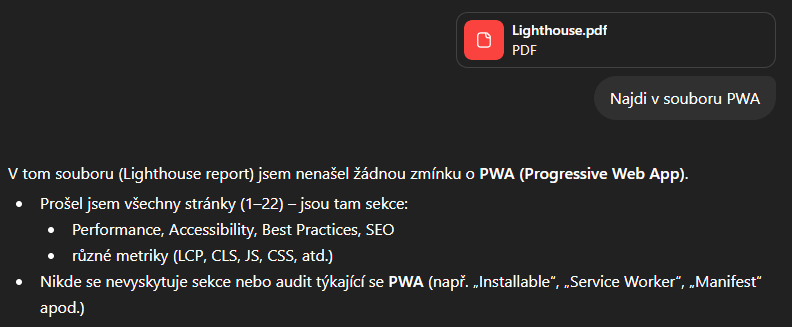
\includegraphics[width=0.92\textwidth]{lighthouse.png}
  \caption{Lighthouse kontrola PWA výstupu. Soubor je uložen jako \texttt{docs/lighthouse.png}.}
\end{figure}

\section{Testování}

Repozitář obsahuje základní automatické testy spustitelné příkazem \texttt{npm test}. Testy používají vestavěný Node.js test runner, samostatný TypeScript build přes \texttt{tsconfig.test.json} a pro React smoke testy programově spuštěný Vite SSR.

Aktuálně automatické testy pokrývají čistou herní logiku v \texttt{src/game/roomActions.ts}:
\begin{itemize}[leftmargin=2em]
  \item ořezání hodnot statů do rozsahu 0--100,
  \item odvozování nálady mazlíčka podle nízkých statů,
  \item detekci stavu na nule nebo pod nulou,
  \item výsledky akcí v místnostech včetně deterministické kontroly kasina.
\end{itemize}

Doplněny jsou také základní integrační smoke testy React rozhraní v \texttt{tests/react-ui.integration.test.mjs}. Ty přes Vite SSR vyrenderují obrazovku výběru mazlíčka a herní obrazovku, a kontrolují, že se v HTML objeví hlavní texty, statistiky, peníze, vybraný mazlíček a akční ovládání.

Při lokální kontrole 27.~4.~2026 dopadly tyto kontroly takto:
\begin{itemize}[leftmargin=2em]
  \item \texttt{npm test} -- prošlo bez chyb, celkem 8 automatických testů,
  \item \texttt{npm run lint} -- prošlo bez chyb,
  \item \texttt{npm run build} -- prošlo, TypeScript i Vite build do \texttt{dist/} byly úspěšné,
  \item \texttt{npm run verify:pwa} -- prošlo, PWA manifest, ikony, HTML odkaz a generovaný service worker byly zkontrolovány.
\end{itemize}

CI workflow na GitHub Actions spouští testy, lint, produkční build a PWA kontrolu před nahráním výstupu na GitHub Pages. Automatické testy pokrývají herní logiku a základní render hlavního React rozhraní, ruční scénáře ale stále ověřují chování v reálném prohlížeči.

Ručně prošlé testovací scénáře:

\subsection*{Scénář 1 -- prázdný start bez uložené hry}
\begin{itemize}[leftmargin=2em]
  \item Vstupní podmínka: v \texttt{localStorage} není žádný klíč \texttt{tamagotchi-wireframe-state}.
  \item Kroky: otevřu aplikaci poprvé.
  \item Očekávaný výsledek: zobrazí se obrazovka pro výběr mazlíčka a tlačítko pro potvrzení bude na začátku neaktivní.
  \item Skutečný výsledek: odpovídá očekávání.
\end{itemize}

\subsection*{Scénář 2 -- pokus pokračovat bez výběru mazlíčka}
\begin{itemize}[leftmargin=2em]
  \item Vstupní podmínka: aplikace je na obrazovce výběru, žádný mazlíček není označen.
  \item Kroky: pokusím se pokračovat bez předchozího výběru.
  \item Očekávaný výsledek: tlačítko \uv{potvrdit výběr} zůstane zablokované a hra se nespustí.
  \item Skutečný výsledek: odpovídá očekávání.
\end{itemize}

\subsection*{Scénář 3 -- výběr mazlíčka a start hry}
\begin{itemize}[leftmargin=2em]
  \item Vstupní podmínka: aplikace je na úvodní obrazovce.
  \item Kroky: vyberu jednoho mazlíčka a kliknu na \uv{potvrdit výběr}.
  \item Očekávaný výsledek: zobrazí se herní obrazovka, aktuální místnost je kuchyň a hráč má 24 peněz.
  \item Skutečný výsledek: odpovídá očekávání.
\end{itemize}

\subsection*{Scénář 4 -- provedení akce v místnosti}
\begin{itemize}[leftmargin=2em]
  \item Vstupní podmínka: hra běží, mazlíček je naživu a hráč má dostatek peněz.
  \item Kroky: v kuchyni kliknu na tlačítko akce.
  \item Očekávaný výsledek: odečtou se peníze, změní se statistiky mazlíčka a přepíše se statusová zpráva.
  \item Skutečný výsledek: odpovídá očekávání.
\end{itemize}

\subsection*{Scénář 5 -- nedostatek peněz}
\begin{itemize}[leftmargin=2em]
  \item Vstupní podmínka: hra běží, ale hráč nemá dost peněz na aktuální akci.
  \item Kroky: přepnu se do dražší místnosti a pokusím se akci spustit.
  \item Očekávaný výsledek: akční tlačítko bude neaktivní, aby nešlo utratit víc peněz, než je k dispozici.
  \item Skutečný výsledek: odpovídá očekávání.
\end{itemize}

\subsection*{Scénář 6 -- časový pokles statů}
\begin{itemize}[leftmargin=2em]
  \item Vstupní podmínka: hra běží na domovské obrazovce.
  \item Kroky: nic neudělám a počkám alespoň 12 sekund.
  \item Očekávaný výsledek: hlad, zdraví, štěstí a energie klesnou podle herních pravidel a změní se statusová zpráva.
  \item Skutečný výsledek: odpovídá očekávání.
\end{itemize}

\subsection*{Scénář 7 -- přechod mezi místnostmi}
\begin{itemize}[leftmargin=2em]
  \item Vstupní podmínka: hra běží a je vidět hlavní karta místnosti.
  \item Kroky: kliknu na levou nebo pravou šipku, případně přejdu z poslední místnosti na první.
  \item Očekávaný výsledek: změní se název, popis, ikona akce i pozadí místnosti; pozadí se plynule posune jako sousední obrazovky.
  \item Skutečný výsledek: odpovídá očekávání.
\end{itemize}

\subsection*{Scénář 8 -- game over}
\begin{itemize}[leftmargin=2em]
  \item Vstupní podmínka: některý stat mazlíčka je těsně nad nulou.
  \item Kroky: nechám běžet hru, dokud jeden stat neklesne na 0.
  \item Očekávaný výsledek: otevře se modal s informací o smrti mazlíčka a hra vyžaduje restart.
  \item Skutečný výsledek: odpovídá očekávání.
\end{itemize}

\subsection*{Scénář 9 -- obnova po reloadu}
\begin{itemize}[leftmargin=2em]
  \item Vstupní podmínka: hra je rozehraná a v \texttt{localStorage} je uložen stav.
  \item Kroky: obnovím stránku v prohlížeči.
  \item Očekávaný výsledek: aplikace načte předchozího mazlíčka, místnost, peníze i poslední stav hry.
  \item Skutečný výsledek: odpovídá očekávání.
\end{itemize}

\subsection*{Scénář 10 -- rozbitá uložená data}
\begin{itemize}[leftmargin=2em]
  \item Vstupní podmínka: v \texttt{localStorage} je schválně vložen nevalidní JSON nebo špatný tvar dat.
  \item Kroky: obnovím stránku.
  \item Očekávaný výsledek: zobrazí se systémová chyba a tlačítko pro nový začátek.
  \item Skutečný výsledek: odpovídá očekávání.
\end{itemize}

\subsection*{Scénář 11 -- světlý a tmavý motiv}
\begin{itemize}[leftmargin=2em]
  \item Vstupní podmínka: aplikace je otevřená a prohlížeč podporuje \texttt{prefers-color-scheme}.
  \item Kroky: kliknu na tlačítko pro přepnutí motivu a potom obnovím stránku.
  \item Očekávaný výsledek: motiv se přepne a po reloadu zůstane uložený.
  \item Skutečný výsledek: odpovídá očekávání.
\end{itemize}

\subsection*{Scénář 12 -- chyba sítě / offline stav}
\begin{itemize}[leftmargin=2em]
  \item Vstupní podmínka: uživatel odpojí internet a chce aplikaci otevřít znovu.
  \item Kroky: vypnu připojení a zkusím obnovit nebo znovu otevřít nasazenou aplikaci.
  \item Očekávaný výsledek: po prvním online načtení by service worker měl umět vrátit app shell a přednačtené assety.
  \item Skutečný výsledek: offline provoz je potřeba ještě ručně ověřit v produkčním prohlížeči.
\end{itemize}

\section{Rozdělení práce}

Z historie větví a commitů je vidět, že práce byla dělena paralelně mezi wireframe/UI část a logickou/infrastrukturní část:

\begin{itemize}[leftmargin=2em]
  \item Martin Veber (Role A -- UI): příprava wireframu, barevného stylu, mobilního layoutu, pet scén, HUD prvků, animací místností, tmavého/světlého vzhledu a finálního vizuálního poladění.
  \item Matyáš Potocký (Role B -- logika): příprava datových typů, výběru mazlíčka, správy stavu, ukládání do \texttt{localStorage}, časové herní smyčky, jednotkových testů, CI, branch protection, nasazení na GitHub Pages a PWA výstupu.
  \item Obě role na sebe navazovaly: nejdřív vznikl wireframe a komponentový základ, potom se doplnila herní logika, persistence a deploy, a nakonec se vzhled znovu doladil včetně animací, testů, PWA zapojení a produkčního buildu.
\end{itemize}

\section{Zhodnocení projektu}

\subsection*{Co se podařilo}

\begin{itemize}[leftmargin=2em]
  \item Podařilo se vytvořit funkční browserovou hru, která má jasný herní cíl a jednoduché ovládání.
  \item Výsledná aplikace působí vizuálně jednotně a mobile-first rozložení je na tak malý projekt nadprůměrně propracované.
  \item Dobře funguje spojení logiky a UI: změny statů se okamžitě projevují v obraze mazlíčka, penězích i informační hlášce.
  \item Praktická je persistence do \texttt{localStorage}, díky které uživatel o rozehranou hru nepřijde po refreshi.
  \item Pozitivní je také to, že projekt má CI workflow, veřejné nasazení na GitHub Pages a aktuálně prochází testy, lint i produkčním buildem.
  \item Povedlo se doplnit plynulý přechod mezi místnostmi, světlý/tmavý motiv, základ PWA, jednotkové testy a React smoke testy.
  \item Kódová základna je uklizenější: staré nepoužívané prototypové komponenty byly odstraněny a README odpovídá aktuální implementaci.
\end{itemize}

\subsection*{Co bylo problematické}

\begin{itemize}[leftmargin=2em]
  \item PWA část je technicky zapojená, má automatickou kontrolu artefaktů a v příloze je doplněný Lighthouse screenshot.
  \item Automatické testy už kontrolují herní logiku i základní render React obrazovek, ale nepokrývají všechny klikací scénáře v reálném prohlížeči.
  \item Pro ještě přesnější kontrolu by šlo doplnit plné prohlížečové end-to-end testy.
\end{itemize}

\subsection*{Co by šlo dále rozvíjet}

\begin{itemize}[leftmargin=2em]
  \item Doložit instalaci PWA ručním testem přímo v prohlížeči.
  \item Rozšířit stávající automatické testy o plné prohlížečové end-to-end scénáře.
  \item Rozšířit hru o další místnosti, více typů akcí, inventář nebo více druhů mazlíčků.
  \item Přidat zvuky, denní odměny, skóre nebo statistiku délky přežití.
  \item Pravidelně udržovat dokumentaci při dalších změnách.
\end{itemize}

\section{Přílohy}

\subsection*{Wireframe z prvního týdne}

Původní wireframe je uložen v repozitáři jako \texttt{docs/wireframe.svg} a pro vložení do zprávy je k dispozici i jako \texttt{docs/wireframe.png}.

\begin{figure}[htbp]
  \centering
  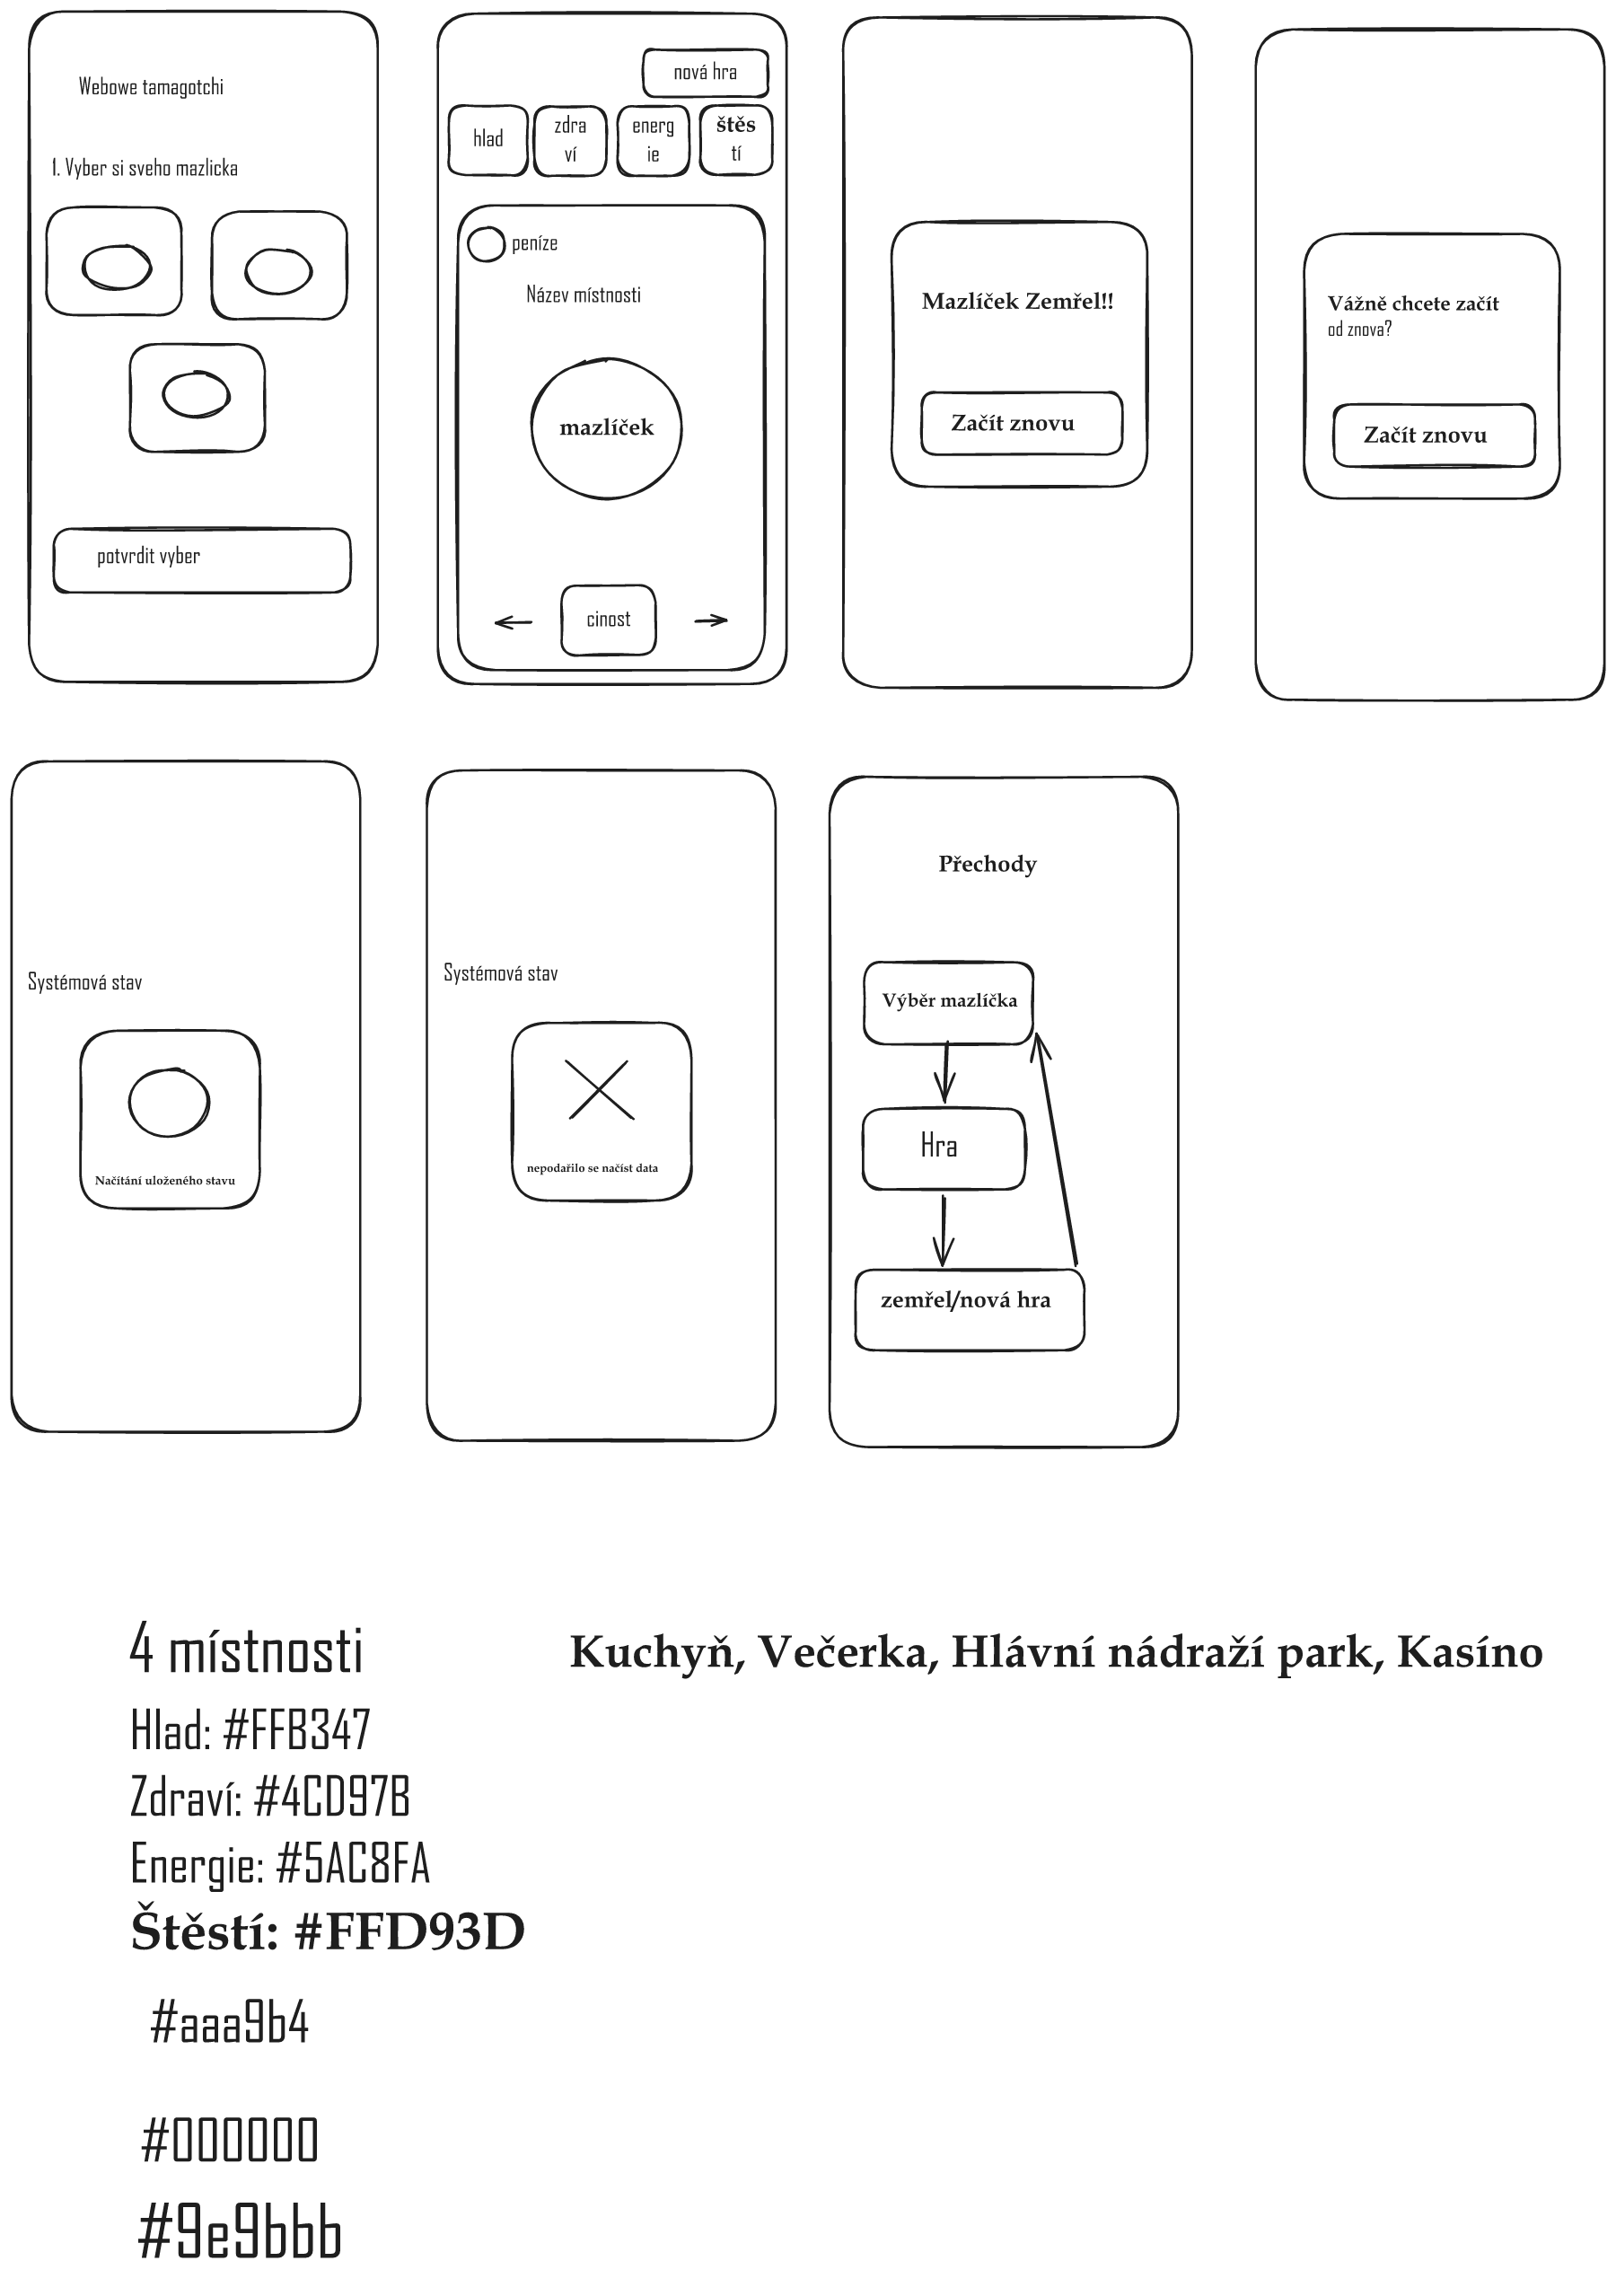
\includegraphics[width=\textwidth]{wireframe.png}
  \caption{Původní wireframe aplikace z prvního týdne vývoje. Soubor je uložen jako \texttt{docs/wireframe.png}.}
\end{figure}

\subsection*{Screenshoty finální aplikace}

V repozitáři jsou uložené screenshoty finální aplikace z mobilní i desktopové šířky. Oba soubory jsou ve složce \texttt{docs/} a slouží jako vizuální doklad aktuálního stavu rozhraní:
\begin{itemize}[leftmargin=2em]
  \item \texttt{docs/obrazovkaHryTelefon.png},
  \item \texttt{docs/obrazovkaHryPocitac.png}.
\end{itemize}

\begin{figure}[htbp]
  \centering
  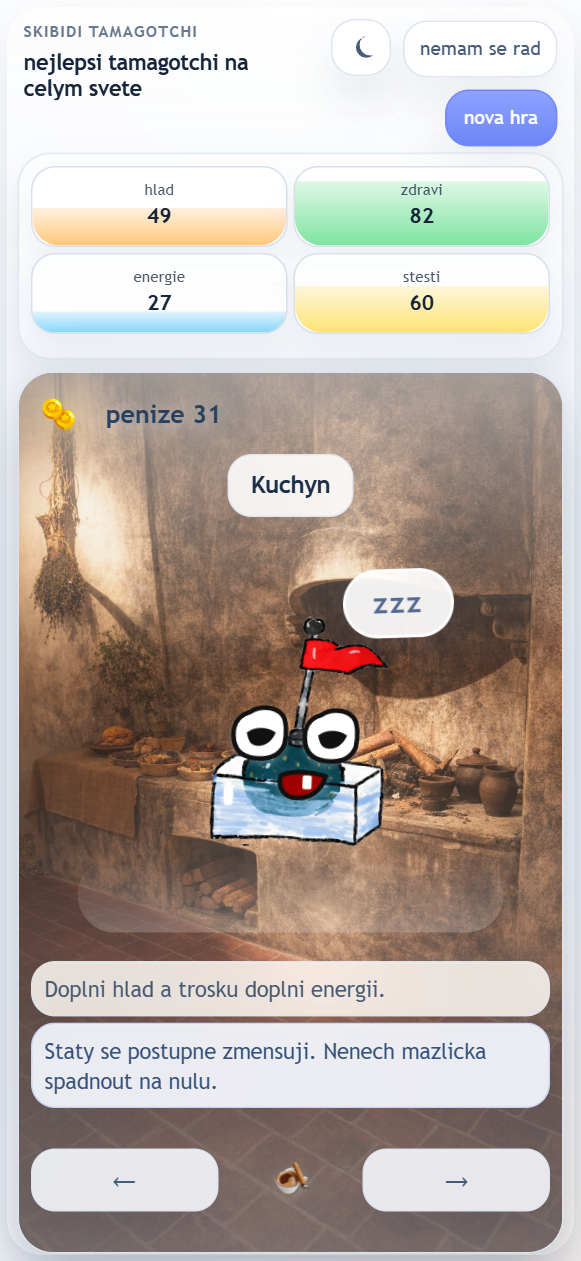
\includegraphics[height=0.72\textheight,keepaspectratio]{obrazovkaHryTelefon.png}
  \caption{Finální aplikace v mobilní šířce. Soubor je uložen jako \texttt{docs/obrazovkaHryTelefon.png}.}
\end{figure}

\begin{figure}[htbp]
  \centering
  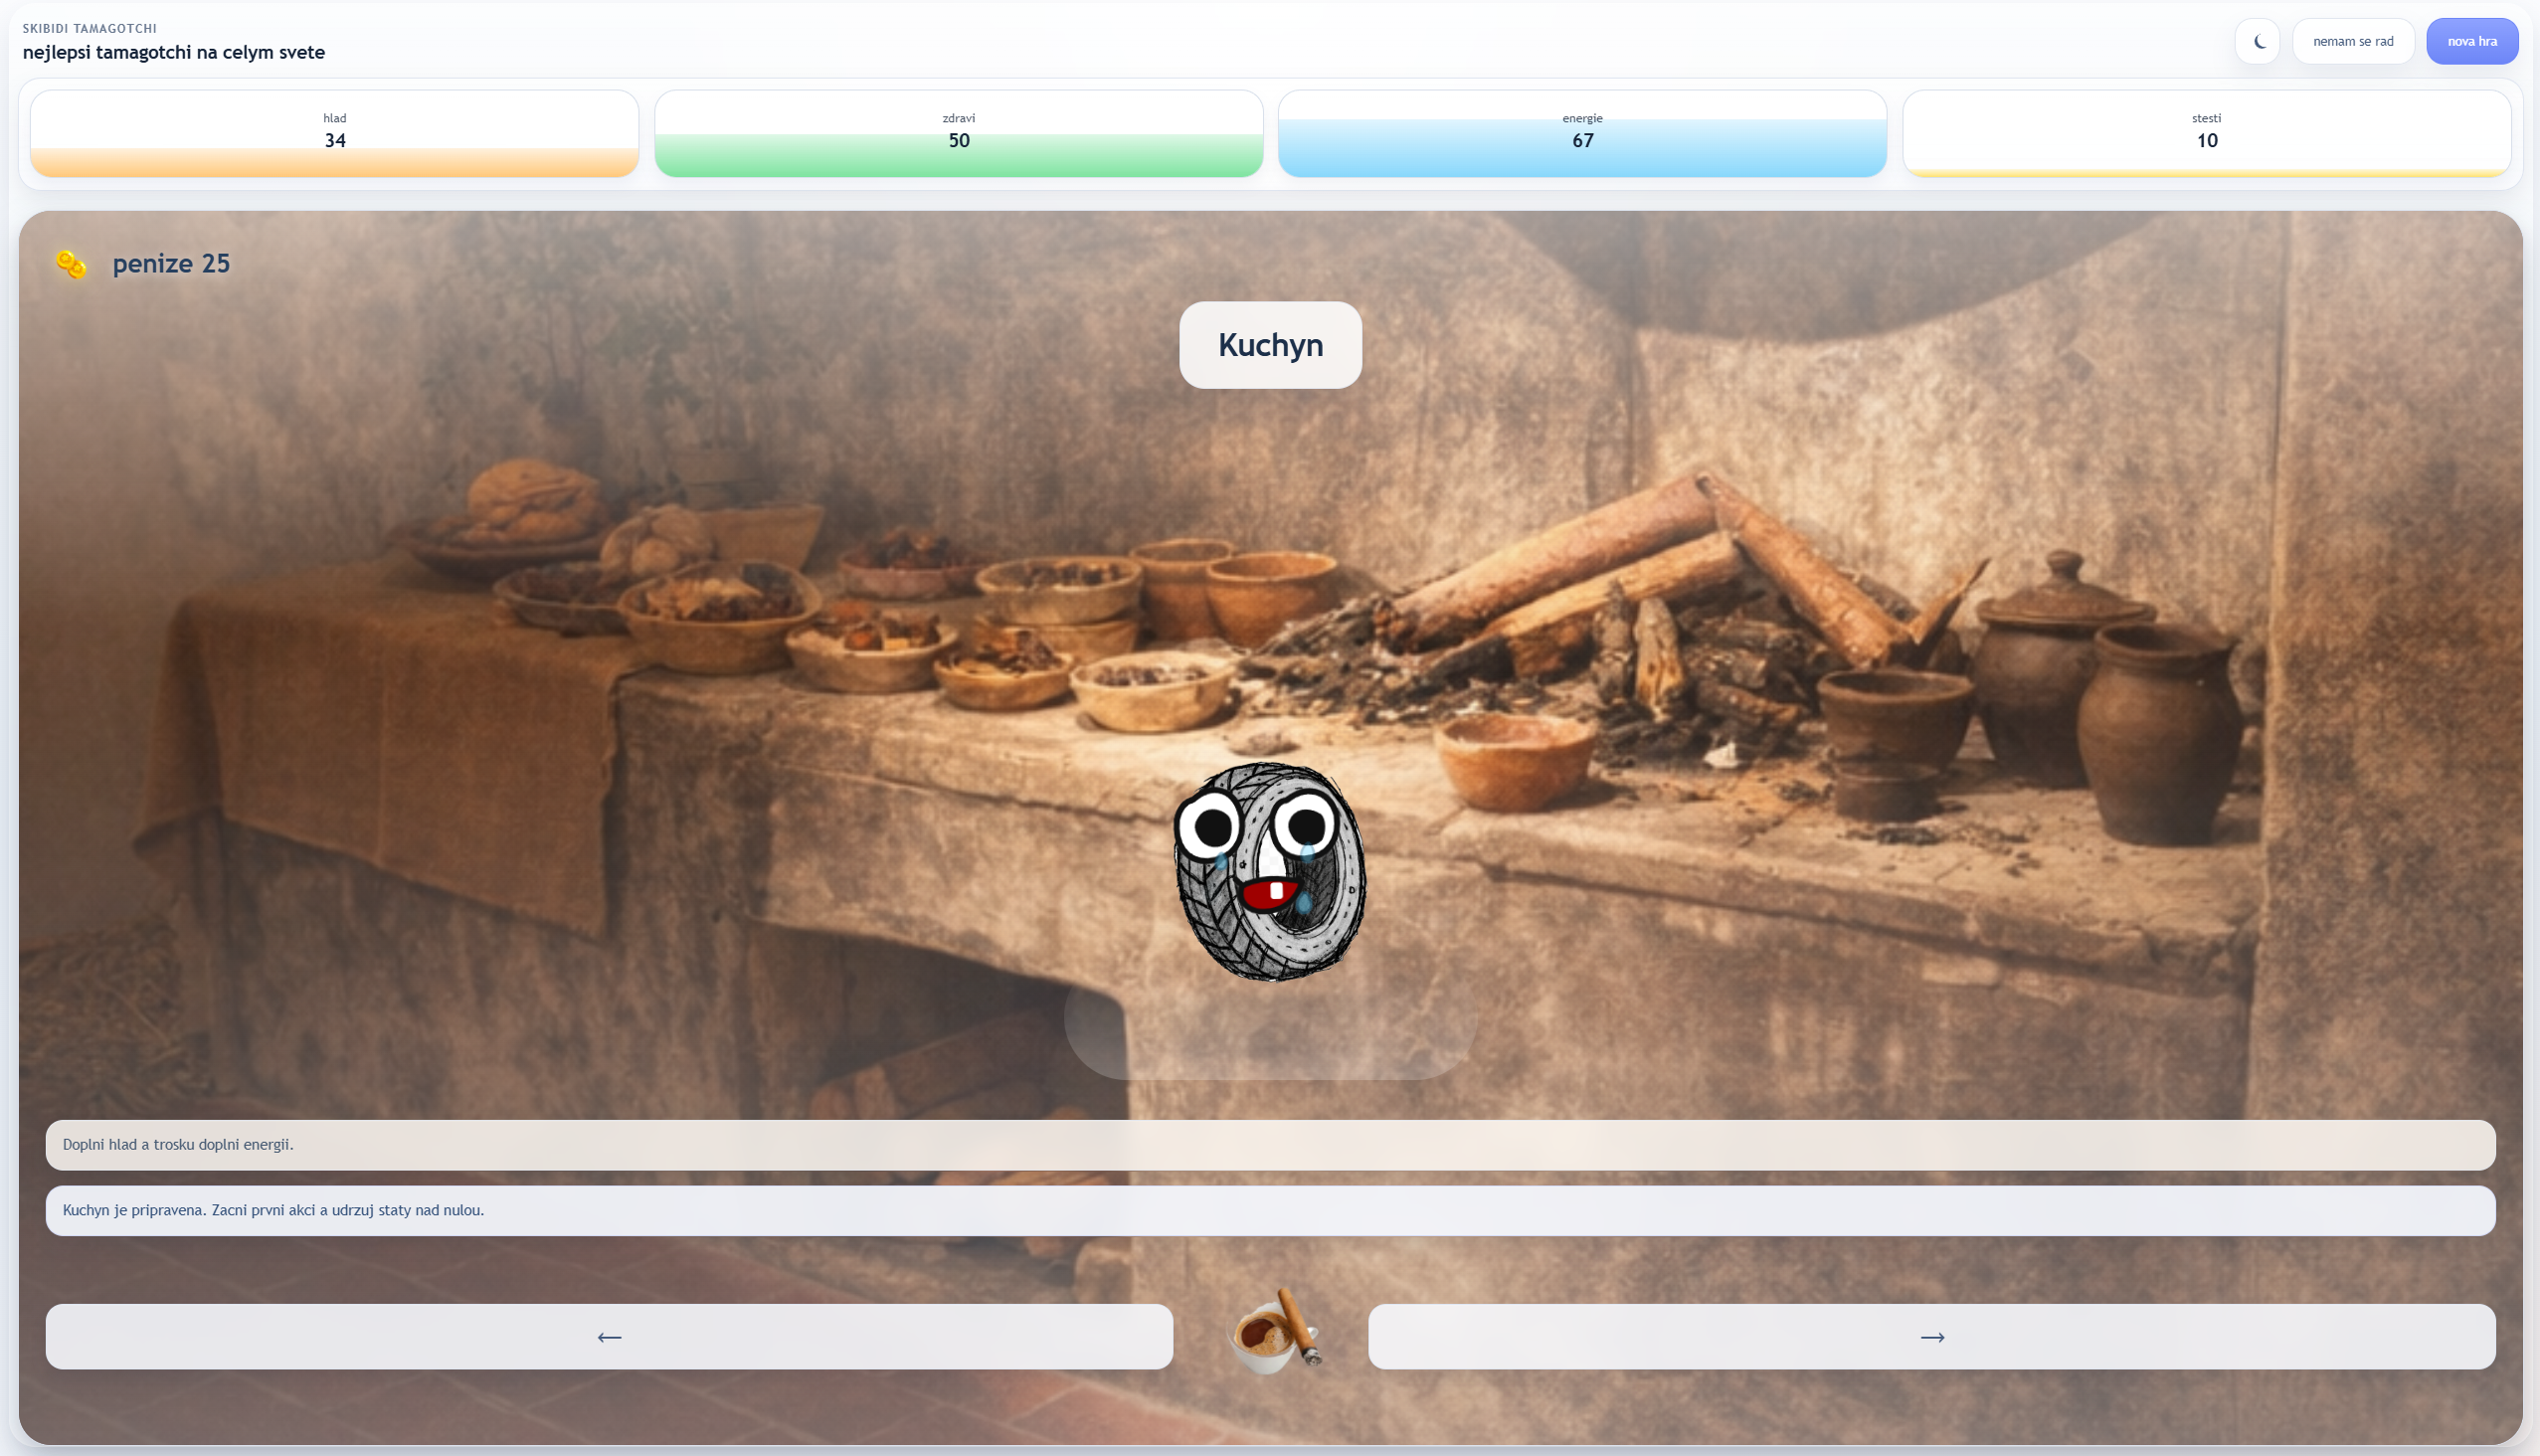
\includegraphics[width=\textwidth]{obrazovkaHryPocitac.png}
  \caption{Finální aplikace v desktopové šířce. Soubor je uložen jako \texttt{docs/obrazovkaHryPocitac.png}.}
\end{figure}

\end{document}
